Data-centric governance means operationalizing performance requirements for AI systems in the form of datasets and algorithmic evaluations to be run against them. It turns abstract requirements like ``fairness'' into objectively measurable phenomena. It recognizes the central role of data in AI system evaluation and the need for good data stewardship and rigorous evaluation protocols to preserve the statistical validity of evaluations against that data.

% Almost all machine learning practitioners know not to train a model on its evaluation data. But for the most part, only in large organizations with substantial machine learning experience are there any significant organizational controls designed to ensure that data is not misused. Such controls are mostly absent from the mid market down, and it is causing problems. 

By one estimate, as many as 85 percent of AI projects fail to deliver or fall short \cite{gartner_predicts_2018}. In our experiences in research and industry, the most common failure point has been failure to appropriately capture the full complexity of the solution's deployment environment and engineer a solution accordingly. As governance processes are often aimed at surfacing potential deployment harms, their systematization earlier in the product lifecycle is likely to substantially reduce the failed delivery rate.

In this section, we lay out the key tasks involved in implementing data-centric governance in practice. Accomplishing these tasks requires a concerted effort from the people involved in all stages of the product lifecycle. We will have more to say about the impact of organizational structure on governance in Section~\ref{sec:teams}. For now, we identify four major areas of responsibility:

\begin{definition}[Product Team]
The people responsible for defining the system's goals and requirements.
\end{definition}

\begin{definition}[Data Team]
The people responsible for collecting and preparing the data necessary for system engineering and evaluation.
\end{definition}

\begin{definition}[Solution Team]
The people responsible for engineering the product.
\end{definition}

\begin{definition}[Verification Team]
The people responsible for ensuring that the solution is consistent with organizational, regulatory, and ethical requirements prior to and following deployment.
\end{definition}

These teams can be staffed by people from a single organization producing a system, or their functions can be represented by external organizations (e.g., auditors can serve as a verification team).

Throughout this section, we will highlight the benefits of effective data-centric governance by contrasting the experiences of these development teams at two fictitious organizations: Governed Corporation (G-Corp), which follows data-centric governance best practices, and Na\"{i}ve Corporation (N-Corp), which does not.


% \begin{figure}[ht]
% \centering
% 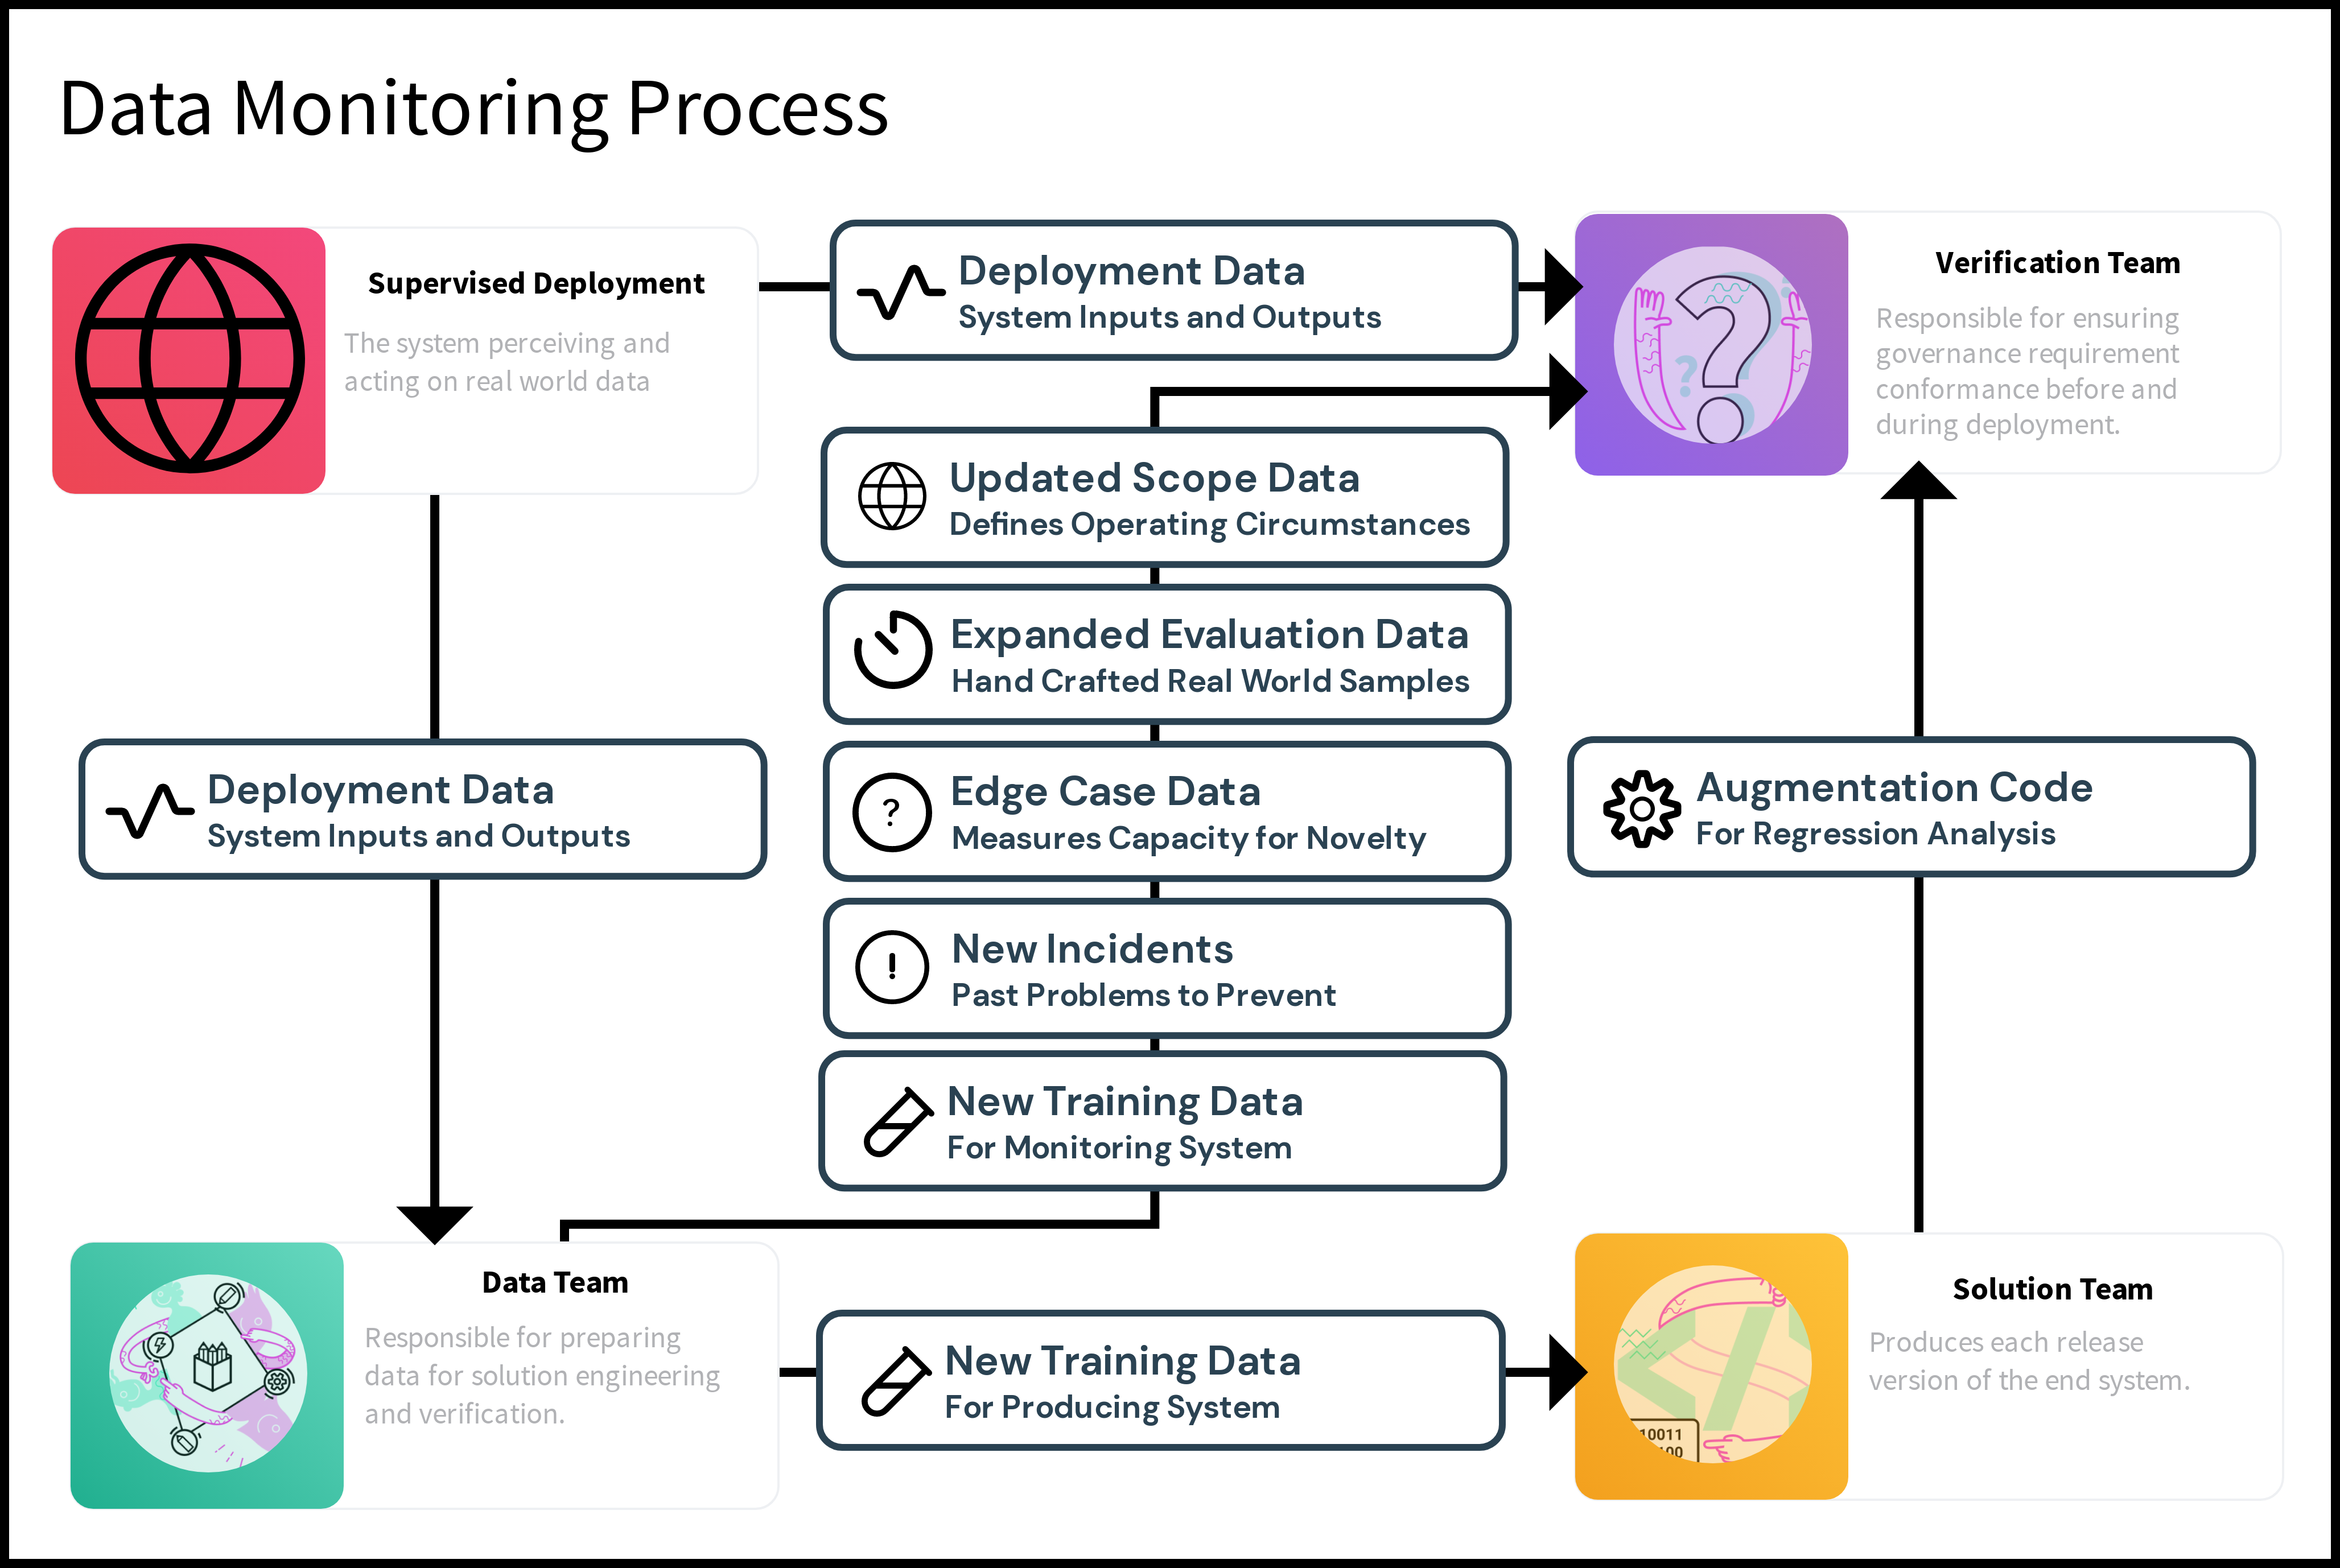
\includegraphics[width=\textwidth]{images/PenpotMonitoring3.png}
% \label{fig:data_monitoring}
% \caption{Data relationships between the system deployment and the teams involved in its production and assurance.}
% \end{figure}

\subsection{Operationalize system requirements} 

Data-centric governance is about turning abstract governance requirements into objectively and algorithmically measurable phenomena. Machine learning practitioners are already familiar with this idea. Test set error, for example, is commonly taken to be the operational definition of task success. But there are many other relevant dimensions of performance. Data-centric governance envisions that measuring the full breadth of relevant performance criteria should be as routine as measuring test set accuracy.

To make this possible, one must specify how to measure performance algorithmically, which for an AI system includes provisioning the evaluation datasets. This creates an objective, repeatable measurement process.  Although emerging requirements at deployment time can necessitate collecting additional evaluation data, performance requirements, like all product requirements, should be defined as early in the development process as possible. Ill-defined requirements are a major cause of project failures in all engineering disciplines, and AI is no exception. 
%The responsibility for requirements definition should, therefore, lie with the Product Team. 
% In our experience, this is rarely done in current practice. It is more 
Nevertheless, it is common for product requirements to be expressed only qualitatively in the design phase, with quantitative measures coming later after significant engineering has already been done. \textbf{This is a harmful practice, as it tends to anchor quantitative requirements to what is measurable with the available data and to the numbers that the chosen engineering approach can achieve.} It is difficult to be objective about what would constitute acceptable performance once expectations are anchored in this way.

Codifying governance requirements with data also enables practitioners to learn from past mistakes. Every AI system incident is an opportunity to identify and formalize a new relevant dimension of performance. Once formalized, it is possible to evaluate future systems for their susceptibility to similar incidents. An AI system's scores on different batteries of data-driven evaluations rigorously characterize the boundaries of its competencies and allow teams to make informed decisions about whether to deploy the system.

\highlight{
\textbf{Contrasting Outcomes}

\paragraph{G-Corp.} The Product Team identifies that the AI system poses a risk of disparate impacts and adds ``fairness across demographic groups'' as a product requirement. They define ``fairness'' as having statistically-equivalent error rates across relevant demographic groups. The Data Team creates engineering and evaluation datasets stratified by demographic groups. The Solution Team optimizes the system to achieve all performance goals on the engineering data. The Verification Team verifies compliance with fairness requirements using the evaluation data and confirms that the system does not produce disparate impacts -- the system is safely deployed.

\paragraph{N-Corp.} The Product Team identifies that the AI system poses a risk of disparate impacts and adds ``fairness across demographic groups'' as a product requirement. The Data Team focuses on engineering and evaluation data for the primary task, and the Solution Team focuses on optimizing for the primary task. The Verification Team checks that the AI system does not use sensitive features as inputs, but has no means of detecting that the model produces disparate impacts because a feature for user location, which was not considered sensitive, is correlated with sensitive attributes. The system is deployed and results in disparate impacts to real-world users.
}

\subsection{Solve the data paradox}

Data-centric governance faces a bootstrapping problem in acquiring the necessary datasets. The reliability of the system cannot be assessed without data that is representative of the actual deployment environment. The obvious way to obtain this data is to collect it from a deployed system. But, without the data, it is impossible to engineer a deployable system or to verify that a release candidate meets its minimum deployment requirements. This is the \emph{data paradox} of data-driven AI systems. The path forward consists of two parts: acquiring realistic proxy data, and expanding the scope of the system iteratively with real deployment data from previous system releases.

\textbf{Acquire realistic proxy data}. Where real-world data is not available, suitably realistic proxy data must be acquired. There are many ways to approach this. For some applications, it may be possible to mine publicly available data collected for other purposes. For example, data for image classification is often sourced from websites like Flickr by searching for relevant keywords. Data that requires more human expertise to generate or label is often obtained from crowdsourcing services like Amazon Mechanical Turk. 

Data collection strategies can be quite elaborate. For example, Google ran a telephone answering service from 2007 to 2010 primarily for the purpose of collecting data for speech-to-text transcription. The sheer amount of effort expended to collect this data should reinforce the value of large, realistic datasets for product creation. Organizations should consider carefully the scale of data required for creating the initial version of the product and the level of realism required, and should budget appropriately for the complexity of acquiring this data.

\textbf{Expand scope iteratively}. Once version 1.0 of a system is created and deployed, it begins to see real-world data from its actual deployment environment. This data should be collected and used to expand the datasets that will be used for creating the next version of the system. Through this bootstrapping process, the solution will gradually improve as larger amounts of real deployment data become available.

The scope of the AI system must be tightly restricted during the initial phases of this bootstrapping process. With limited deployment data available, the scope within which the system's competencies can be verified through evaluation data is also limited, and therefore it must be prevented from operating in circumstances where the risk of harm cannot be measured. The scope of the system should begin small and expand gradually, informed by continuing evaluations of performance in the real deployment environment.

% \highlight{
% \textbf{Does this mean we can deploy an ungoverned system?} 

% Google's Pixel phones, all major voice agents, drone suppliers, Tesla's cars, and more, all have deployed hardware to the world without turning on the full capabilities of the systems. After appropriate engineering and evaluation data are produced in the field, new features can activate following measured compliance with governance requirements.

% \takeaway{A restricted system, even one that takes no actions, can bootstrap the cycle of measurement and improvement without undue risk.}}

\highlight{
\textbf{Contrasting Outcomes}

\paragraph{G-Corp.} The Product Team produces a grand vision for a device that will change the world and plans shipments to 30 countries. The Data Team finds appropriate data sourced from a single country and the Solution Team begins engineering. Knowing the data will not support shipments to 30 countries, the Go2Market strategy shifts to running pilot programs with the production device in 29 of the 30 markets. The Verification Team signs off on shipping to 1 country and the product is a huge hit -- driving enrollment in the pilot program in the remaining 29 countries.

\paragraph{N-Corp.} The Product Team produces a grand vision for a product that will change the world and justifies its multi-million dollar development budget on shipments to 30 countries. The Data Team finds appropriate data sourced from a single country and the Solution Team begins engineering. The Verification Team then is overruled when attempting to block shipments to all but the represented country. N-Corp is worried G-Corp will be first-to-market. After poor performance in 29 of the 30 markets (including several newsworthy incidents), the product is recalled globally -- including in the one strong-performing market.
}

\subsection{Steward the data}

Implementing data-centric governance requires that some entity take responsibility for data stewardship. This includes collecting and storing the data, making it available for evaluations while guarding it against misuse, and performing data maintenance activities to ensure the continued construct validity of data-centric measures as the application domain changes. Data stewardship is a shared responsibility of the Data Team and the Verification Team. The Data Team decides what data is needed to measure a given construct and how to obtain it, and the Verification Team ensures that evaluations against the data are conducted properly.

\textbf{Preserve diagnostic power}. Exposing evaluation data to Solution Teams compromises the validity of evaluations based on that data. Even if Solution Teams exercise proper discipline in not training on the test data, something as innocent as comparing evaluation scores of multiple models can be a step down the road to overfitting \cite{blum_ladder_2015}. Practitioners may not be aware of all of the subtleties of statistically rigorous evaluation, and even when they are, some of the more ``pedantic'' requirements may be seen as unnecessary impediments to speedy delivery of a solution. 

There is also the practical problem that without data access controls, it is not possible to \emph{verify} that the evaluation data has not been misused. This is especially important when the evaluation is an ``industry standard'' benchmark, where showing state-of-the-art performance may bring prestige or financial benefits. The Verification Team is responsible for facilitating data-driven evaluations in a way that preserves the validity of the evaluation data as a diagnostic tool. The evaluation data must be kept private and the release of evaluation scores must be controlled so as not to reveal information about the data \cite{blum_ladder_2015}.

\highlight{
\textbf{Contrasting Outcomes}

\paragraph{G-Corp.} The Data Team creates evaluation datasets that are collected independently of all engineering datasets. The Data Team delivers the evaluation data to the Verification Team and does not disclose the data or the method of collection to the Solution Team. The Solution Team passes their trained models off to the Verification Team, which evaluates the systems and reports the results in a way that avoids disclosing information about the evaluation data. The organization can be confident that the solution has not overfit the evaluation data, and thus that the evaluation results are reliable.

\paragraph{N-Corp.} The Data Team delivers both the engineering data and the evaluation data to the Solution Team. The Solution Team knows the risks of overfitting the evaluation data, but under pressure to improve performance, they make changes to improve the model guided by its scores on the evaluation data. The Verification Team verifies that the system meets performance requirements and approves it for deployment. The system under-performs after deployment because architecture changes driven by repeated evaluations resulted in overfitting the evaluation data.
}

\textbf{Maintain the data}. The world changes over time, and with it changes the distribution of inputs that a deployed AI system will be asked to process. A computer vision system that tracks vehicles on the road, for example, will see new vehicle models introduced throughout its lifetime \cite{dietterich_familiarity_2022}. Evaluation data must be \emph{maintained} to ensure that it continues to be a valid operational measure of the associated performance requirement. This will usually require, at least, periodically collecting additional data, and possibly also pruning obsolete data or designing new data augmentations.

Data maintenance is a joint activity of the Data Team and the Verification Team. The Verification Team should conduct ongoing evaluations to look for signs of domain shift and alert the Data Team when additional evaluation data is needed. This likely requires collaboration with the Solution Team to ensure that the system emits the necessary diagnostic information after deployment. Once alerted, the Data Team should create new or modified datasets and pass them back to the Verification Team for integration into the evaluation process. 

\highlight{
\textbf{Contrasting Outcomes}

\paragraph{G-Corp.} A development team is creating an image classification app meant to run on smartphones. Whenever a new model of smartphone is released by a major manufacturer, the Data Team collects engineering and evaluation datasets comprised of images of a standard set of subjects captured with the new model of phone. Periodic system revisions include data from new phone models in their engineering and evaluation data. The app maintains high performance over time.

\paragraph{N-Corp.} After deployment of the first version of the app, the Data Team considers their work complete and moves on to other projects. The app begins to perform poorly with the latest models of the phone. The Solution Team attempts to improve the model, but improving performance on the existing data seems to make performance with the new phones even worse. Users of newer phone models stop using the app because of its poor performance.
}

\textbf{Evaluation Authorities}. In many instances data stewardship is best performed by evaluation authorities tasked with assessing system impact requirements. Evaluation authorities standardize entire product categories with independent measurements. For example, stamped on the bottom of most AC adapters are the letters "UL Listed," which stands for Underwriters Laboratories -- an organization that has worked to test and standardize electrical safety since 1894. Without organizations like UL, electricity would be far too dangerous to embed in the walls of all our homes and businesses. People will not buy electrical systems in the absence of electrical standards. Similarly, intelligent systems are often not purchased because the purchaser has no way of efficiently and reliably determining the capacities of the system.

\highlight{
\textbf{Contrasting Outcomes}

After producing Résumé screening apps that are measurably far fairer than any human screener, G-Corp and N-Corp find they cannot sell their products to anyone because nobody trusts the performance numbers. Both firms engage third party auditors to evaluate the technology.

\paragraph{G-Corp.} G-Corp pays the auditor a nominal premium on their normal audit price to subsequently serve as an ``evaluation authority'' for the market segment. As the first public standard of its kind, the entire human resources industry soon standardizes around it and G-Corp develops a performance lead from having been there first.

\paragraph{N-Corp.} N-Corp's solution performs just as well as G-Corp's, but their measures are soon rendered irrelevant after other competitors standardize to the G-Corp audit. Since competitors cannot compare against N-Corp's numbers, G-Corp wins the market.
}

\subsection{Adopt continuous assurance}

As software engineering practice has shown, the best way to ensure that requirements are met is to verify them automatically as a matter of course after every system modification and throughout the lifecycle of the system. In analogy to the continuous integration and continuous deployment (CI/CD) paradigm that has transformed the practice of software engineering, we need \emph{continuous assurance} practices for AI system engineering. This section lays out the core components of continuous assurance; we discuss tooling for continuous assurance in Section~\ref{sec:outline_systems}.

\textbf{Extend CI/CD to AI systems}. The components of continuous assurance for AI systems mirror the components of CI/CD in many respects. Both CI and CD gate development and release via test suites analogous to evaluation data. To utilize the test suite, the system must be designed for testability. For an AI system, this means that the system in its deployable form must expose a generic interface enabling it to consume data from arbitrary sources and produce results. The system should also be modular with loose coupling among components so that components can be tested separately. Unfortunately, modern machine learning techniques have trended toward ``end-to-end'' monolithic models that are difficult to separate into components. The reason for this trend is that such models often perform somewhat better than modular architectures, but solution engineers must be aware that this performance comes at the price of testability. Recent interest in ``explainable AI'' is in part a reaction to this trend, acknowledging the need to understand the intermediate computational steps implicit in the model.

In addition to testable models, we need the computational infrastructure to run the tests at scale. This is already a well-known pain point in CI/CD, and there are many companies offering solutions like cloud-based distributed build and test systems. The problem may be even more acute for AI systems due to the computational expense of running large evaluation datasets. Such problems can be overcome, but organizations developing AI systems must understand the problems and plan and budget accordingly.

Finally, just like CI/CD, continuous assurance requires an associated versioning system for AI models. Because AI models are products of training on data, the versioning system must also track versions of the training data and other parameters of the training pipeline, and record which version of the training inputs produced which version of the model.

\highlight{
\textbf{Contrasting Outcomes}

\paragraph{G-Corp.} The development teams implement a continuous assurance process in which deployment candidate models are checked in after training and run against the evaluation suite automatically. This allows them to notice that the new version of the model, which has more parameters, has better task performance but is less robust to noise. The Solution Team improves the model by adding regularization, and the improved model passes all evaluations.

\paragraph{N-Corp.} The Verification Team conducts performance evaluations in the traditional way, by receiving the model from the Solution Team and manually performing \textit{ad hoc} evaluations. They note its improved performance on the primary task evaluation data, but they do not run the noise robustness tests because these take extra effort and they were run for the previous model version. The model is deployed, where it performs poorly in noisy environments.
}

\textbf{Monitor deployed systems and report incidents}. While the data-centric governance practices we have discussed so far offer teams the best chance of deploying reliable, trustworthy systems, training and verification data will always be incomplete, and the world will always continue to change after the AI system is deployed. AI systems therefore require ongoing monitoring after deployment. 

One objective of ongoing monitoring is to detect and report excursions from the AI system's proper operating scope as they happen. Techniques like out-of-distribution detection should be applied to compare real-world inputs and outputs to those in the engineering and evaluation datasets. Departures from the expected distributions of data could mean that the system is operating in novel regimes where it may not be reliable. Timely detection of these departures can allow human decision-makers to place limits on the system or withdraw it from operation if its reliability cannot be guaranteed.

A second objective is to collect real-world inputs and outputs so that they can be used to augment and improve engineering and evaluation datasets. Real-world edge cases and incidents should be tracked to build edge case and incident datasets so that the system can be improved to handle these cases. Continuous assurance processes should incorporate acquired real-world data to ensure that revisions of the AI system handle new edge cases and incidents and do not regress in their handling of known cases. Accumulating real-world data also guards against domain shift by ensuring that engineering and evaluation datasets are up-to-date with the changing world.

\highlight{
\textbf{Contrasting Outcomes}

\paragraph{G-Corp.} The Solution Team developing a wake word detection system includes an out-of-distribution (OOD) detection component in the system. During deployment, the OOD detector sends an email alert to the Verification Team indicating that the input data distribution is substantially different from the evaluation data distribution. By analyzing the real-world data collected by the system, the Verification Team determines that the engineering and evaluation datasets do not contain enough variation in speaker accents. They report this to the Data Team, who use the collected data to build more-diverse datasets, improving performance of the next system revision.

\paragraph{N-Corp.} Without any monitoring components in place, the developer teams are unaware that the deployed system is operating with a different input distribution than the ones used for engineering and evaluation. Their first indication is when customers with certain accents begin reporting poor performance to customer service. The developers eventually realize the problem, but because data from the deployed system was not collected, the Data Team must collect more-diverse data in a lab setting, at considerable expense. Some customers who were frustrated by poor performance switch to a competitor's product.
}
